\documentclass[PublicacaoDissOuTese, PublicacaoLivro, brazilian]{dissertacaoUFGpac}
%\documentclass[PublicacaoDissOuTese, brazilian]{tdiinpe}
\usepackage{graphics}\graphicspath{{./figs/}} %Define figures place

\hyphenation{co-lo-car pa-la-vra pa-ra hi-fe-ni-zar}

%\watermark{RASCUNHO} %% use o comando \watermark para identificar a vers�o de seu documento
% comente este comando quando for gerar a vers�o final

%%%%%%%%%%%%%%%%%%%CAPA%%%%%%%%%%%%%%%%%%%%%%%%%%%%%%%%
\instituicao{UNIVERSIDADE~FEDERAL~DE~GOI�S}
\instituicaol{PROGRAMA~DE~P�S-GRADUA��O~EM ENGENHARIA~EL�TRICA E~DE~COMPUTA��O}
\instituicaosigla{[UFG] \& [EMC]}
\instituicaocidade{[Goi�nia - Goi�s - Brasil]}

\author{Bernardo Araujo Rodrigues} %% coloque o nome do(s) autor(es)
\email{bernardoaraujor@gmail.com}

%\titulo{Controlador Preditivo baseado em Modelo N�o Linear Sintonizado por Algoritmo Gen�tico Aplicado ao Controle de Velocidade de M�quina de Corrente Cont�nua Acionada por Retificador Trif�sico Controlado: An�lise Comparativa com Controlador PI Cascata Sintonizado por Algoritmo Gen�tico} %% no idioma principal
\titulo{Corinda: Quebrando Hashes de Senhas Concorrentemente com a Linguagem Go}
\date{\today}

\descriccao{
  Disserta��o apresentada a Banca Examinadora como exig�ncia parcial para a
   obten��o do t��tulo de Mestre em Engenharia El�trica e de Computa��o pela
   Universidade Federal de Goi�s (UFG), Escola de Engenharia El�trica,
   Mec�nica e de Computa��o (EMC), sob a orienta��o do Prof. Dr. Wesley
   Pacheco Calixto.
}

\tituloverso{\vspace{-0.9cm}\textbf{}}
\descriccaoverso{}

%%%%%%%%%%%%%%%%%%%FOLHA DE ROSTO
\descriccaoversoA{}
\instituicao{UNIVERSIDADE~FEDERAL~DE~GOI�S}
\instituicaol{PROGRAMA~DE~P�S-GRADUA��O~EM ENGENHARIA~EL�TRICA E~DE~COMPUTA��O}
\instituicaosigla{[UFG] \& [EMC]}
\instituicaocidade{[Goi�nia - Goi�s - Brasil]}

\author{Bernardo Araujo Rodrigues} %% coloque o nome do(s) autor(es)
\email{bernardoaraujor@gmail.com}

%\titulo{Controlador Preditivo baseado em Modelo N�o Linear Sintonizado por Algoritmo Gen�tico Aplicado ao Controle de Velocidade de M�quina de Corrente Cont�nua Acionada por Retificador Trif�sico Controlado: An�lise Comparativa com Controlador PI Cascata Sintonizado por Algoritmo Gen�tico} %% no idioma principal
\titulo{Corinda: Quebrando Hashes de Senhas Concorrentemente com a Linguagem de Programa��o Go}
%\title{Nonlinear Model Predictive Controller Tuned by Genetic Algorithm Applied do Direct Current Motor Speed Control Triggered by Three Phase Controlled Rectifier: Comparative Analysis with Cascade PI Controller Tuned by Genetic Algorithm} %% no idioma secundario
\title{Corinda: Cracking Password Hashes with Go Programming Language}
\date{\today}
%\serieinpe{} %% ser� determinado pela biblioteca posteriormente

\descriccao{Disserta��o apresentada a Banca Examinadora como exig�ncia parcial para a
   obten��o do t��tulo de Mestre em Engenharia El�trica e de Computa��o pela
   Universidade Federal de Goi�s (UFG), Escola de Engenharia El�trica,
   Mec�nica e de Computa��o (EMC), sob a orienta��o do Prof. Dr. Wesley
   Pacheco Calixto.}

%%%%%%%%%%%%%%%FICHA CATALOGR�FICA

\cutterFICHAC{C331s}
\autorUltimoNomeFICHAC{Rodrigues, Bernardo Araujo, 31/07/90} %% exemplo: Fuckner, Marcus Andr�
\autorAbreviadoFICHAC {Rodrigues, B. A.} %% N�o usado - deixar vazio
\tituloFICHAC{Corinda: Quebrando \textit{Hashes} de Senhas Concorrentemente com a Linguagem de Programao Go [manuscrito]}
\paginasFICHAC{\pageref{LastPage} f. : il}%% n�mero total de p�ginas
\palavraschaveFICHAC{Orientador: Wesley Pacheco Calixto - UFG\\\\
Disserta��o - Universidade Federal de Goi�s - UFG, Escola de Engenharia El�trica, Mec�nica e de Computa��o - EMC\\\\
Inclui bibliografia.\\\\
1.Senhas - Teses. 2.\textit{Hashes} - Teses. 3.Seguran�a da Informa��o - Teses.  I. Calixto, Wesley
Pacheco; II. Universidade Federal de Goi�s.  Programa de P�s-Gradua��o em Engenharia El�trica e de Computa��o. III. Corinda: Quebrando \textit{Hashes} de Senhas Concorrentemente com a Linguagem de Programao Go
} %% recomenda-se pelo menos 5 palavras-chaves - \mbox{} � para evitar hifeniza��o
\numeroCDUFICHAC{000.0.000:000.0} %% n�mero do CDU

%%%tdiinpe
%%%%%%%%%%%%%%%%%%%%%%%%%%%%%%%%%%%%%%%%%%%%%%%%%%%%%%%%%%%%%%%%%%%5
%\titulo{titulo}
%\descriccao{descriccao}
%
%\repositorio{repositorio}
%\tipoDaPublicacao{tituloDaPublicacao}
%\IBI{IBI}
%
%\email{email}
%\instituicao{instituicao}
%\instituicaol{instituicaol}
%\instituicaosigla{instituicaosigla}
%\instituicaocidade{instituicaocidade}
%
%\tituloverso{tituloverso}
%\descriccaoverso{descriccaoverso}
%\descriccaoversoA{descriccaoversoA}
%
%% FICHA
%
%\cutterFICHAC{cutterFICHAC}
%\autorUltimoNomeFICHAC{autorUltimoNomeFICHAC}
%\autorAbreviadoFICHAC{autorAbreviadoFICHAC}% n�o usado nesse .cls
%\autorFICHAC{autorFICHAC}
%\tituloFICHAC{tituloFICHAC}
%\paginasFICHAC{paginasFICHAC}
%\numeroFICHAC{numeroFICHAC}
%\palavraschaveFICHAC{palavraschaveFICHAC}
%\numeroCDUFICHAC{numeroCDUFICHAC}
%\nomeAtributoOrientadorFICHAC{nomeAtributoOrientadorFICHAC}
%\valorAtributoOrientadorFICHAC{valorAtributoOrientadorFICHAC}
%
%% Nota da ficha (para TD)
%
%\tipoTD{tipoTD}
%\instituicaoDefesa{instituicaoDefesa}
%\anoDefesa{anoDefesa}
%
%% FICHA - fim
%
%\marcaRegistrada{marcaRegistrada}
%
%\tituloFA{tituloFA}
%\cursoFA{cursoFA}
%\candidatoOUcandidataFA{candidatoOUcandidataFA}
%\dataAprovacaoFA{dataAprovacaoFA}
%\membroA{membroA}{mebroAP}{membroAPC}
%\membroB{}{}{}
%\membroC{}{}{}
%\membroD{}{}{}
%\membroE{}{}{}
%\membroF{}{}{}
%\membroG{}{}{} %% fa�a as modifica��es pertinentes no arquivo configuracao.tex

\makeindex  %% n�o alterar, gera INDEX, caso haja algum termo indexado no texto

\begin{document} %% in�cio do documento %% n�o mexer

\maketitle

%%%%%%%%%%%%%%%%%%%%%%%%%%%%%%%%%%%%%%%%%%%%%%%%%%%%%%%%%%%%%%%%%%%%%%%
% Ep�grafe %% opcional

\begin{epigrafe} %% insira sua ep�grafe abaixo; estilo livre

\hypertarget{estilo:epigrafe}{} %% uso para este Guia

\textit{\large``Escreva aqui a ep�grafe.''}

\vspace{1cm}

\hspace{4cm} \emph{\textsc{Escreva aqui o nome do autor da ep�grafe}}\\\hspace{4cm}
%em \textsl{``New York Times''}, March 13, 1940.

\end{epigrafe} %% opcional
%%%%%%%%%%%%%%%%%%%%%%%%%%%%%%%%%%%%%%%%%%%%%%%%%%%%%%%%%%%%%%%%%%%%%%%%%%%%%%%%
% Dedicat�ria %% opcional

\begin{dedicatoria} %% insira sua dedicat�ria abaixo; estilo livre

\hypertarget{estilo:dedicatoria}{} %% uso para este Guia

%% use 'a meus' em vez de 'aos meus', isto �, n�o use o artigo definido com pronomes possessivos

\newcommand{\mytext}{Escreva aqui sua dedicat�ria.}

%%% sugest�o de estilo
\ifcalligra %% fonte calligra presente nas vers�es mais novas do MiKTeX (>= 2.4)
  \calligra\Large \mytext %% exemplo usando estilo de fonte caligr�fica, caso haja
\else
	\itshape\Large \mytext
\fi

\end{dedicatoria}
 %% opcional
%%%%%%%%%%%%%%%%%%%%%%%%%%%%%%%%%%%%%%%%%%%%%%%%%%%%%%%%%%%%%%%%%%%%%%%%%%%%%%%%
% AGRADECIMENTOS %% opcional

\begin{agradecimentos}  %% insira abaixo seus agradecimentos

\hypertarget{estilo:agradecimentos}{} %% uso para este Guia

Escreva aqui seus agradecimentos...
\end{agradecimentos}


 %% opcional
%%%%%%%%%%%%%%%%%%%%%%%%%%%%%%%%%%%%%%%%%%%%%%%%%%%%%%%%%%%%%%%%%%%%%%%%%%%%%%%%
% RESUMO %% obrigat�rio

\begin{resumo} %% insira seu resumo abaixo

\hypertarget{estilo:resumo}{} %% uso para este Guia

Escreva aqui o resumo do seu trabalho...

\end{resumo}


 %% obrigat�rio
%%%%%%%%%%%%%%%%%%%%%%%%%%%%%%%%%%%%%%%%%%%%%%%%%%%%%%%%%%%%%%%%%%%%%%%%%%%%%%%%
% ABSTRACT


\begin{abstract} %% insira abaixo seu abstract

\hypertarget{estilo:abstract}{} %% uso para este Guia

Write here the abstract of your work ...

\end{abstract}


 %% obrigat�rio

\includeSumario  %% obrigat�rio, gerado automaticamente
\includeListaFiguras %% obrigat�rio caso haja mais de 3 figuras, gerado automaticamente
\includeListaTabelas %% obrigat�rio caso haja mais de 3 tabelas, gerado automaticamente

%%%%%%%%%%%%%%%%%%%%%%%%%%%%%%%%%%%%%%%%%%%%%%%%%%%%%%%%%%%%%%%%%%%%%%%%%%%%%%%%%
%% lista de simbolos
%o comando: \hypertarget{estilo:simbolos}{} pode ser retirado
%%%%%%%%%%%%%%%%%%%%%%%%%%%%%%%%%%%%%%%%%%%%%%%%%%%%%%%%%%%%%%%%%%%%%%%%%%%%%%%%%55
\begin{simbolos} %retirar o coment�rio dessa linha se ocorrerem s�mbolos na sua tese ou disserta��o. N�o esque�a de atualizar o publica��o.tex
\hypertarget{estilo:simbolos}{}

Coloque seus s�mbolos aqui conforme exemplo:\\\\
%$$ &--& \\
$N_m$ 	 &--& Horizonte do modelo\\
$N_u$		 &--& Horizonte de controle\\
$N_y$ 	 &--& Horizonte de predi��o\\
$\alpha$ &--& Taxa de amortecimento da refer�ncia\\
$\omega$ &--& Trajet�ria refer�ncia\\

\end{simbolos}


%%%%%%%%%%%%%%%%%%%%%%%%%%%%%%%%%%%%%%%%%%%%%%%%%%%%%%%%%%%%%%%%%%%%%%%%%%%%%%%%%
%% siglas e abreviaturas  %% opcional, mas recomendado
%

%%%%%%%%%%%%%%%%%%%%%%%%%%%%%%%%%%%%%%%%%%%%%%%%%%%%%%%%%%%%%%%%%%%%%%%%%%%%%%%%%%%%%%%%%%%
%%% sigla (separador: &--&) significado (quebra de linha: \\)
%
%%% o comando: \hypertarget{estilo:siglaseabreviaturas}{} abaixo pode ser retirado
 %%%%%%%%%%%%%%%%%%%%%%%%%%%%%%%%%%%%%%%%%%%%%%%%%%%%%%%%%%%%%%%%%%%%%%%%%%%%%%%%%%%%%%%%%%%
\begin{abreviaturasesiglas}  %% retirar o coment�rio dessa linha se ocorrerem abreviaturas e siglas na sua tese ou disserta��o. N�o esque�a de atualizar o publica��o.tex
\hypertarget{estilo:abreviaturasesiglas}{}

&& Coloque suas abreviaturas aqui conforme exemplo.\\\\

AG     &--& Algoritmo Gen�tico\\
CA		 &--& Corrente Alternada\\
CC		 &--& Corrente Cont�nua\\
CMD    &--& Controle por Matriz Din�mica\\
CPBM   &--& Controle Preditivo Baseado em Modelos\\
CPBML  &--& Controle Preditivo Baseado em Modelo Linear\\
CPBMNL &--& Controle Preditivo Baseado em Modelo N�o Linear\\
CPPNL  &--& Controle Preditivo Pr�tico N�o Linear\\
CPG    &--& Controle Preditivo Generalizado\\
IAE    &--& Integral do valor absoluto do erro\\
ISE    &--& Integral do erro quadr�tico\\
ITAE   &--& Integral do valor absoluto do erro multiplicado pelo tempo\\
MCC    &--& Motor de Corrente Cont�nua\\
MIMO   &--& Sistemas Multivari�veis\\
PID		 &--& Proporcional, Integral e Derivativo\\
SISO   &--& Sistemas Monovari�veis\\
%

%SABPR &--& Secretaria da Agricultura e\\ %% significado muito grande
%        && do Abastecimento do Paran�\\ %% ocupa mais de uma linha
\end{abreviaturasesiglas}


\inicioIntroducao

%%%%%%%%%%%%%%%%%%%%%%%%%%%%%%%%%%%%%%%%%%%%%%%%%%%%%%%%%%%%%%%%%%%%%%%%
% CAP�TULO 1
\chapter{INTRODU��O (xx/02/2018)}\label{chapter:introducao}

Conceitos como Internet das Coisas, Computa��o na Nuvem e Redes Sociais possuem papel
cada vez mais fundamental no desenvolvimento social e econ�mico da sociedade atual. Isso faz com que o tema da Seguran�a da Informa��o seja cada vez mais importante \cite{hutchens_2014}. Com isto, qualquer vulnerabilidade inerente a uma tecnologia amplamente utilizada torna-se alvo de interesse ao p�blico em geral.

\par Senhas s�o objetos importantes em sistemas computacionais, sendo essenciais para 
garantir a seguran�a de informa��es pessoais ou sigilosas, bem como acesso a variedade de dispositivos inteligentes \cite{cisar_cisar_2007}.
Enquanto diversos tipos alternativos de autentica��o t�m sido implementados, 
senhas baseadas em sequ�ncias de caracteres ainda s�o o tipo de autentica��o mais comum \cite{shen_khanna_1997, singh_yamini_2013, jayamaha_2008, zhang_koushanfar_2016}.

\par Combina��es fr�geis de \textit{username} e senhas fazem com que dispositivos e contas sejam facilmente comprometidas por agentes maliciosos \cite{florencio_herley_2007, dellamico_michiardi_roudier_2010, bishop_klein_1995}. Al�m de senhas fracas, a reutiliza��o de senhas � pr�tica comum entre usu�rios \cite{gaw_felten_2006}. Tais pr�ticas abrem espa�o para t�cnicas de engenharia social e escalada de privil�gios, tais como as utilizadas no vazamentos de dados do servi�o de armazenamento de arquivos \textit{Dropbox} em 2016, onde agentes maliciosos se aproveitaram de senhas reutilizadas para obter acesso ao sistema da empresa \cite{conger_lynley_2017}.

\par Fun��es de dispers�o criptogr�ficas (FDC) geram longa e complexa sequ�ncia de caracteres (chamada \textit{hash}) a partir de informa��o inicial, sendo matematicamente imposs�vel recuperar a informa��o original a partir do \textit{hash} calculado, permitindo que tal informa��o seja armazenada secretamente. FDC s�o fun��es unidirecionais, o que significa que a �nica forma de obter determinado \textit{hash} � fornecendo a informa��o original como entrada da fun��o \cite{menezes_2001, stallings_2017}. Atualmente, sistemas computacionais armazenam apenas o \textit{hash} da senha do usu�rio. A autentica��o ocorre quando o \textit{hash} calculado a partir da senha digitada pelo usu�rio � comparada com o \textit{hash} armazenado no banco de dados, permitindo o acesso caso os valores sejam iguais \cite{menezes_2001}.

\par No contexto de modelagem de amea�as, o indiv�duo malicioso tentando obter a senha em quest�o � chamado de atacante. O administrador do sistema ou especialista que tenta previnir que a senha seja comprometida � chamado de defensor \cite{swiderski_snyder_2009}. De forma a obter a senha, o atacante deve encontrar a sequ�ncia de caracteres cuja FDC corresponde ao \textit{hash} roubado do banco de dados. Tal processo de adivinha��o � chamado de quebra da senha, e existem ferramentas espec�ficas capazes de realizar milh�es de palpites por segundo, tais como \textit{John The Ripper} e \textit{Hashcat} \cite{murakami_kasahara_saito_2010, hashcat_2016}. \textit{Hashcat} � a ferramenta mais avan�ada e popular atualmente, tornando poss�vel o uso de t�cnicas de paraleliza��o baseadas no uso de \textit{Open Computing Language} (\textit{OpenCL}), descrita por \citeonline{munshi_2009}. O \textit{Hashcat} pode ser utilizado em diversas plataformas de \textit{hardware}, tais como Unidades de Processamento Central (\textit{CPU}), Unidades de Processamento Gr�fico (\textit{GPU}), Processadores Digitais de Sinais (\textit{DSP}), e Arranjos de Portas Program�veis em Campo (\textit{FPGA}).

\par T�cnicas de quebra de senhas tem sido amplamente pesquisadas, n�o apenas pela comunidade cient�fica, mas tamb�m por comunidades online e f�runs \cite{weir_2009, bishop_klein_1995, wang_2016}. Em 2016, mais de $96\%$ dos \textit{hashes} vazados dos bancos de dados da rede social de neg�cios \textit{LinkedIn}, descritos por \citeonline{gosney_2016}, foram quebrados menos de cinco meses depois de terem sido disponibilizados online. Se as senhas forem simples o bastante, mesmo FDC robustas n�o resitem a t�cnicas modernas de quebra de senha.

\par Quando usu�rios criam suas senhas, a maioria tende a utilizar padr�es que possam ser facilmente lembrados. Isto faz com que seja poss�vel que o atacante consiga adivinh�-la. Alguns autores trabalharam com a tentativa de encontrar padr�es na forma que os usu�rios criam suas senhas. \citeonline{weir_2009} utilizam gram�ticas probabil�sticas livre de contexto como entrada em \textit{software} de quebra de senha. \citeonline{bishop_klein_1995} procuram por padr�es comuns tais como n�meros de caracteres e palavras de dicion�rios. Outros pesquisadores tamb�m tentaram elaborar m�tricas confi�veis capazes de quantificar o qu�o robusta determinada senha � frente a tentativas de quebra. \citeonline{castellucia} utilizam Modelos de Markov para modelar a for�a de senhas. O padr�o definido por \citeonline{burr, burr2} nas diretrizes de autentica��o online do \textit{National Institute of Standards and Technology} (\textit{NIST}) prop�e a entropia de caractere como m�trica de for�a. \citeonline{kelley2} avaliam a m�trica do \textit{NIST} como �til, por�m limitada na maioria dos casos. \citeonline{kelley1} prop�em como m�trica a entropia emp�rica baseada em senhas previamente coletadas, tamb�m com resultados limitados.

\par De forma a estabelecer \textit{framework} generalizado para a quantifica��o da resist�ncia de determinada senha contra t�cnicas de quebra, \citeonline{sahin} formaliza os conceitos de \textbf{complexidade} e \textbf{for�a} com s�lidas defini��es matem�ticas que enfatizam suas diferen�as. Estes conceitos possuem import�ncia fundamental no contexto de quebra de senhas, uma vez que eles derivam da compreens�o fundamental de que:

\begin{citacao}
 \textit{...o sucesso do atacante ao quebrar uma senha deve ser definido pelos seus recursos computacionais dispon�veis, tempo dispon�vel, FDC utilizada, bem como a topologia que define o espa�o de busca \cite{sahin}}.
\end{citacao}

\par Com o objetivo de avaliar os conceitos de complexidade e for�a estabelecidos por \citeonline{sahin}, \citeonline{rodrigues} realizam s�rie de experimentos. Entre as conclus�es, observa-se que existem padr�es estat�sticos distintos na distribui��o das senhas analisadas. A possibilidade de cria��o de m�trica que reflita tais padr�es estat�sticos, bem como o conceito de complexidade estabelecido por \citeonline{sahin}, justificam este estudo.

\begin{itemize}
	\item Hip�tese
	\item Objetivos
	\item Estrutura do trabalho
\end{itemize} %% Cap�tulo 1
%%%%%%%%%%%%%%%%%%%%%%%%%%%%%%%%%%%%%%%%%%%%%%%%%%%%%%%%%%%%%%%%%%%%%%%%
% CAP�TULO 2
\chapter{CONTROLE MODERNO (xx/xx/2017)}\label{chapter:cap2}

\section{Controle cl�ssico e moderno}

Aqui voc� deve escrever umas 15 linhas ou mais sobre a diferen�a entre controles cl�ssicos e controle moderno. Termine citando os controladores por modos deslizantes e o preditivo.

\section{Controle por modos deslizantes}

Aqui voc� deve falar do controle por modos deslizantes.

\subsection{Sintonia do controlador por modos deslizantes}

Aqui voc� deve dar �nfase nas vari�veis manipuladas do controle por modos deslizantes.

\section{Controle preditivo baseado em modelos}

Aqui voc� deve falar do controle preditivo baseado em modelos.

\subsection{Sintonia do controlador preditivo baseado em modelos}

Aqui voc� deve dar �nfase nas vari�veis manipuladas do controle preditivo baseado em modelos.

\section{Considera��es}

Veja as Figura~\ref{Exep1} e Figura~\ref{Exep2}, que servem de exemplo para inser��o figuras.

\begin{figure}[!h]
	\centering
	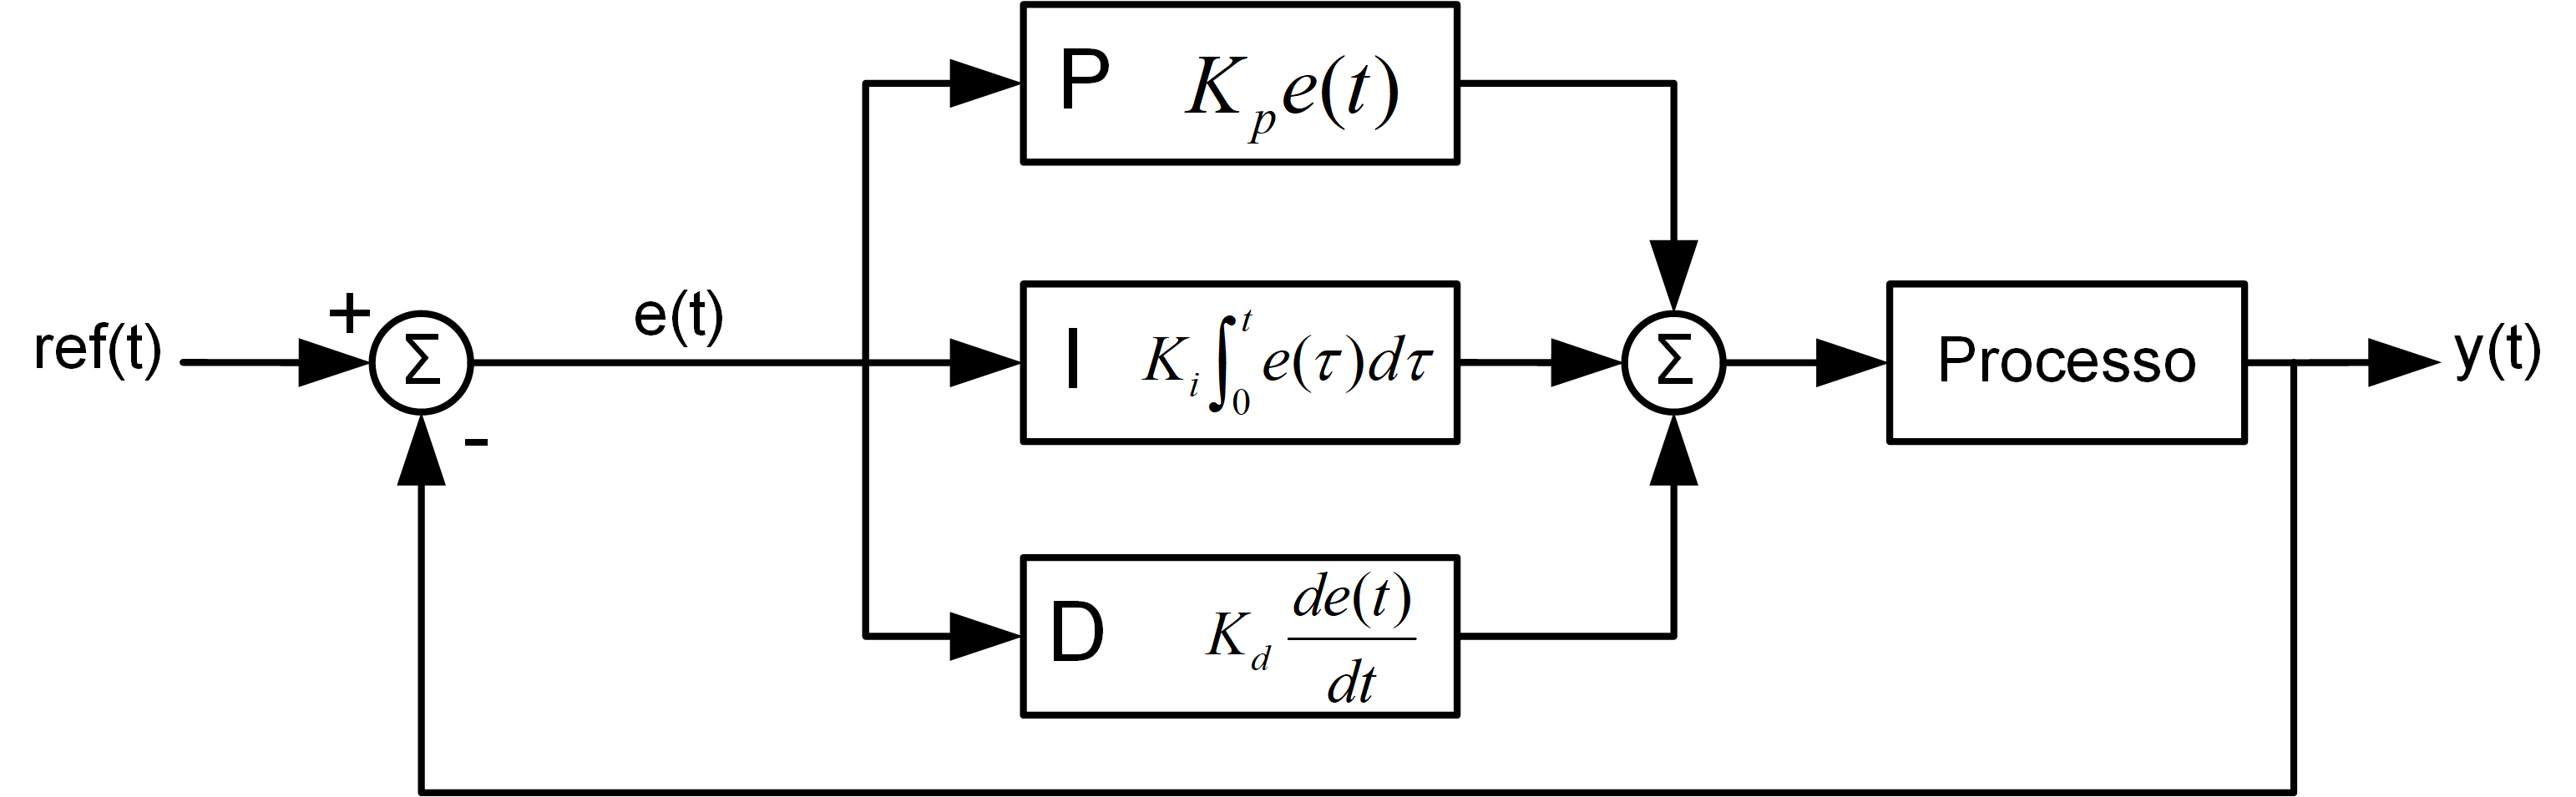
\includegraphics[width=20pc]{./figs/Fig1-1}
	\caption{Partes construtivas do motor de corrente cont�nua.}
	\label{Exep1}
\end{figure} 

\begin{figure}[!h]
	\begin{center}
		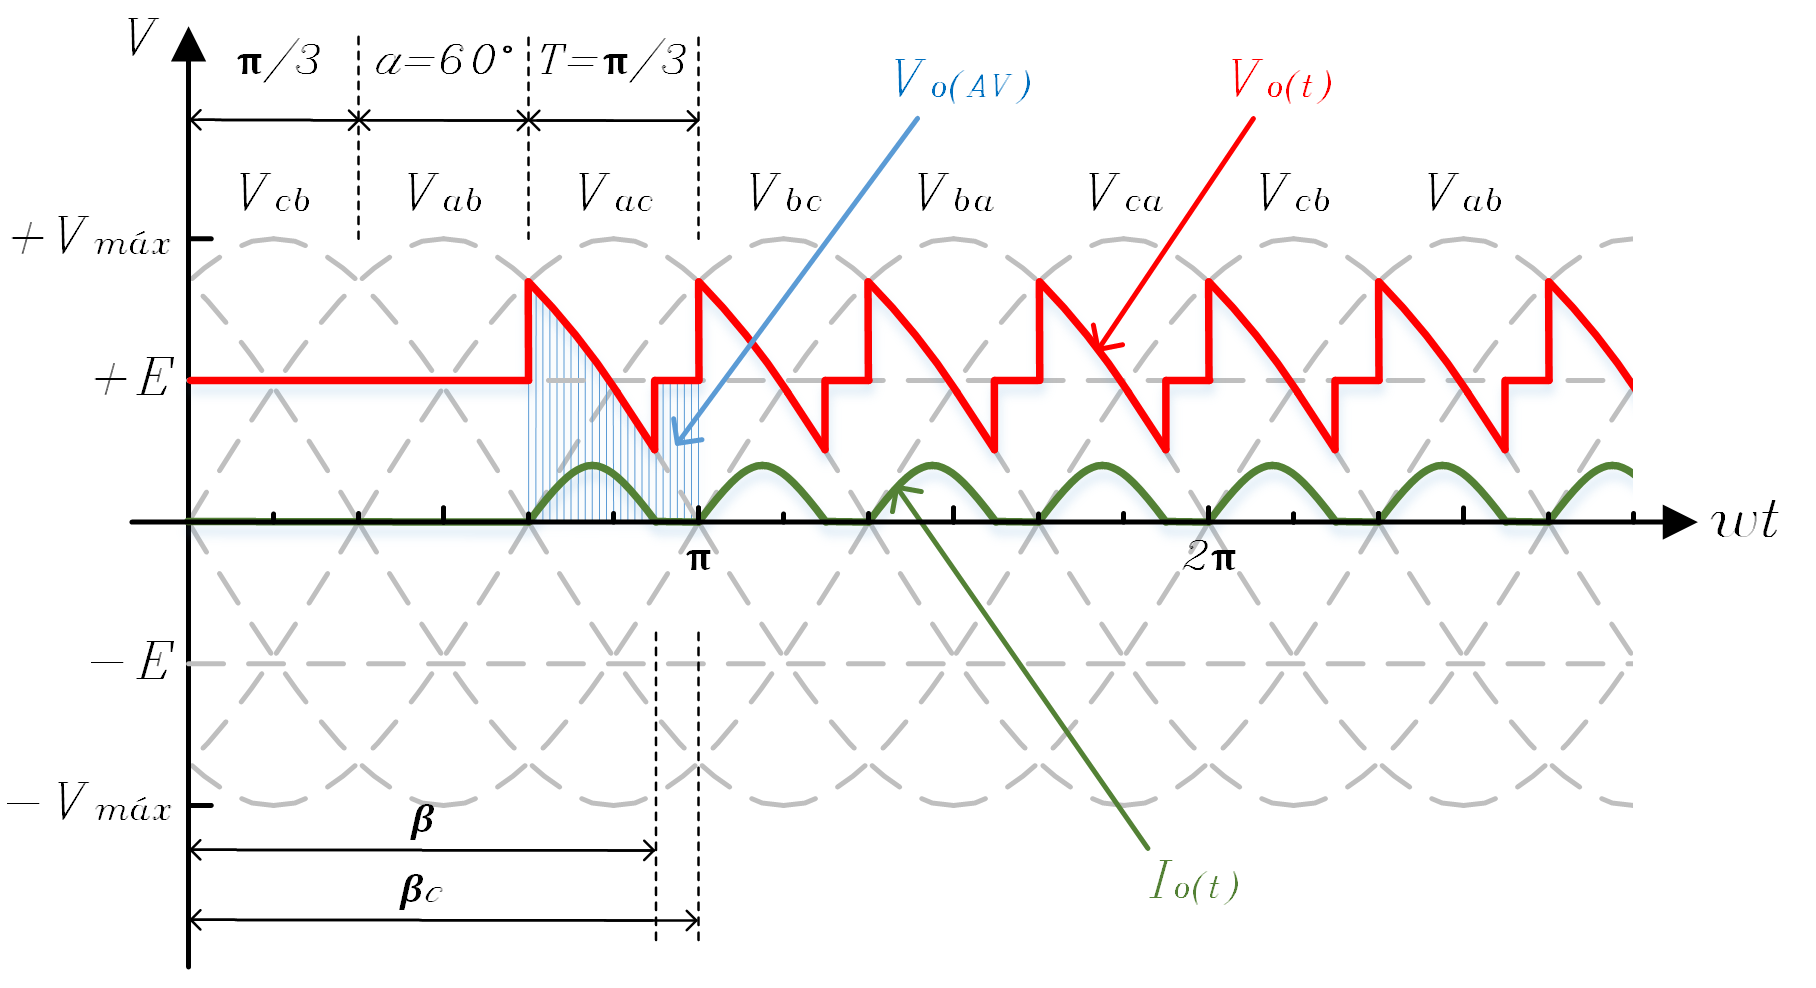
\includegraphics[width=\linewidth]{./figs/Fig2-4}
		\caption{Liga��es de m�quinas CC: (a) excita��o independente, (b) em deriva��o, (c) em s�rie, (d) composta.}
		\label{Exep2}
	\end{center}
\end{figure} %% Cap�tulo 2
%%%%%%%%%%%%%%%%%%%%%%%%%%%%%%%%%%%%%%%%%%%%%%%%%%%%%%%%%%%%%%%%%%%%%%%%
% CAP�TULO 3
\chapter{SISTEMA, MODELO E OTIMIZA��O (xx/xx/2017)}\label{chapter:cap3}

\section{Sistema}

Aqui voc� deve definir o que � sistema. Pode utilizar o livro do Medina e outros.

\section{Modelo}

Aqui voc� deve definir o que � modelo. Pode utilizar o livro do Medina e outros.

\subsection{Constru��o da modelagem do motor de corrente cont�nua}

Aqui voc� deve falar somente o necess�rio para que seu leitor entenda o que � o modelo do motor de corrente cont�nua, dado as express�es que o define.

\section{Processo de otimiza��o}

Aqui voc� deve falar sucintamente sobre o processo de otimiza��o. Pegue o material comigo.

\subsection{Otimiza��o aplicada ao controle do motor de corrente cont�nua}

Aqui voc� fala do trabalho do M�rcio, Douglas e Rafael, descrevendo o que eles fizeram como processo de otimiza��o.

\section{Considera��es}

Veja as express�es (\ref{Equ1}) e (\ref{Equ2}), que servem de exemplo de como inserir express�es matem�tica.

\begin{equation}
v_{a}(t) = R_{a}\cdot i_{a}(t) + L_{a} \frac{di_{a}(t)}{dt} + e_{g}(t)
\label{Equ1}
\end{equation}

\begin{equation}
v_{f}(t) = R_{f}\cdot i_{f}(t) + L_{f} \frac{di_{f}(t)}{dt}
\label{Equ2}
\end{equation} %% Cap�tulo 4
%%%%%%%%%%%%%%%%%%%%%%%%%%%%%%%%%%%%%%%%%%%%%%%%%%%%%%%%%%%%%%%%%%%%%%%%
% CAP�TULO 4
\chapter{METODOLOGIA (xx/xx/2017)}\label{chapter:cap4}

\section{Constru��o e configura��o do sistema}

\section{Modelagem e simula��o}

\section{Aplica��o do processo de otimiza��o na sintonia dos controladores}

\section{An�lise de desempenho entre os controladores}

\section{Considera��es}

 %% Cap�tulo 5
%%%%%%%%%%%%%%%%%%%%%%%%%%%%%%%%%%%%%%%%%%%%%%%%%%%%%%%%%%%%%%%%%%%%%%%%
% CAP�TULO 5
\chapter{RESULTADOS (xx/xx/2018)}\label{chapter:cap5}

Se qualifica��o, \textbf{RESULTADOS PRELIMINARES}. Se defesa final, apenas \textbf{RESULTADOS}.

Na mesma sequ�ncia da metodologia.

\section{Constru��o da bancada e do modelo}

\section{Resultado de simula��o}

\subsection{Otimiza��o aplicada na sintonia dos controladores}

\section{Resultado de bancada}

\section{Coment�rios}

Veja as Tabela~\ref{Tab1} e Tabela~\ref{Tab2}, que servem de exemplo de como inserir tabela. Caso necess�rio, baixe o aplicativa \textit{La Table} para lhe auxiliar na formata��o de tabelas.

\begin{table}[h!]
	\centering
	{\footnotesize 
		\caption{Par�metros da express�o NARMAX do modelo do sistema.}
		\begin{tabular}{c|l}
			\hline
			\hline
			\textbf{Par�metro} & \textbf{Valores}\\		        \hline\hline
			$n_y$ & $\begin{bmatrix} 1 \\ \end{bmatrix}$\\	
			$n_u$ & $\begin{bmatrix} 1 \\ \end{bmatrix}$\\		
			$t_d$ & $\begin{bmatrix} 1 \\ \end{bmatrix}$\\		
			$P$ & $\begin{bmatrix}
			0.0011 & -0.0032 \\
			3.97\cdot 10^{-6} & 0.0872 \\
			\end{bmatrix}$\\                             		
			$L'$ & $\begin{bmatrix} 928.9889 & 14.3086 \\ \end{bmatrix}$\\		\hline\hline
			$d$ & $\begin{bmatrix} 1338.6041 \\ \end{bmatrix}$\\         		
			$Q$ & $\begin{bmatrix}
			0.0011 & -0.0032 \\
			3.97\cdot 10^{-6} & 0.0872 \\
			\end{bmatrix}$\\		
			$A$ & $\begin{bmatrix} -248.3902 & -39.8336 & 27.1611 & 12.6842 & 28.3081 \\ \end{bmatrix}$\\
			$B$ & $\begin{bmatrix}
			-2.0417 & 4.9036 & 3.2205 & 4.0505 & 5.7625 \\
			0.9853 & 1.0024 & -0.9176 & -0.8418 & 0.4071 \\
			\end{bmatrix}$\\
			$C$ & $\begin{bmatrix} 8.9914 & -8.2400 & -6.0503 & -4.3234 & -1.7206 \\ \end{bmatrix}$\\		\hline\hline
	\end{tabular}}
	\label{Tab1}
\end{table}


\begin{table}[h!]
	\centering
	\caption{Par�metros otimizados para o controlador PID.}
	\begin{tabular}{c|c|c|c}
		\hline
		\hline
		\textbf{Par�metro} & $K_P$ & $K_I$ & $K_D$\\
		\hline
		\textbf{Valores} & $0,01241$ & $0,000002$ & $0,00641$\\
		\hline
		\hline
	\end{tabular}
	\label{Tab2}
\end{table}
 %% Cap�tulo 6
%%%%%%%%%%%%%%%%%%%%%%%%%%%%%%%%%%%%%%%%%%%%%%%%%%%%%%%%%%%%%%%%%%%%%%%%
% CAP�TULO 6
\chapter{CONCLUS�O (xx/xx/2018)}\label{chapter:cap6}

Se qualifica��o, \textbf{CONCLUS�O PARCIAL}. Se defesa final, apenas \textbf{CONCLUS�O}.

\section{Contribui��es do Trabalho}
As contribui��es podem assim ser descritas:

\textbf{Artigos em revista:}

\textbf{Artigos em congresso:}

\textbf{Se qualifica��o:}
\section{Continua��o do trabalho}\label{Sec62}

\textbf{Se defesa final:}
\section{Sugest�es para Trabalhos Futuros}\label{Sec63}

 %% Cap�tulo 7


\inicioAnexo
%\include{./docs/anexo1}%% insira anexos com este comando

\bibliography{./bib/publicacao} %% aponte para seu arquivo de bibliografia no formato bibtex (p.ex: publicacao.bib)
\hypertarget{references}{}
%%%%%%%%%%%%%%%%%%%%%%%%%%%%%%%%%%%%%%%%%%%%%%%%%%%%%%
%Gloss�rio
\hypertarget{estilo:glossario}{} %% uso para este Guia
%%%%%%%%%%%%%%%%%%%%%%%%%%%%%%%%%%%%%%%%%%%%%%%%%%%%%%
\begin{glossario}
\label{glossario}
\item[Condutiv�metro] - � um medidor digital port�til que mensura a condutividade el�trica do solo diretamente "\emph{in loco}".

\item[Data Logger] - � um coletor de dados tamb�m chamado de datalogger ou gravador de dados. � um dispositivo eletr�nico que registra os dados ao longo do tempo ou em rela��o a uma localiza��o, constru�do com sensores externos. S�o baseados em um processador digital com mem�rias internas para armazenamento de dados. S�o de uso geral para uma gama de aplica��es em dispositivos de medi��o espec�ficos, podem ser program�veis.

\item[GPS] - � um sistema de navega��o por sat�lite que fornece a um aparelho receptor m�vel a posi��o do mesmo, assim como informa��o hor�ria, sob todas quaisquer condi��es atmosf�ricas, a qualquer momento e em qualquer lugar na Terra, desde que o receptor se encontre no campo de vis�o de quatro sat�lites GPS.

\item[Neossolo Regol�tico] - s�o tipos de solos que apresentam textura arenosa e baixa capacidade de adsor��o de nutrientes, quando comparado com solos argilosos, possui baixo teor de mat�ria org�nica e nitrog�nio que diminuem, ap�s alguns anos de uso agr�cola.

\item[Nitossolo Vermelho] - s�o solos minerais, n�o-hidrom�rficos, apresentando cor vermelho-escura tendendo � arroxeada. S�o derivados do intemperismo de rochas b�sicas e ultrab�sicas, ricas em minerais ferromagnesianos. Uma caracter�stica peculiar � que esses solos, como os Latossolos Roxos, apresentam materiais que s�o atra�dos pelo im�. Seus teores de ferro ($Fe2O3$) s�o elevados (superiores a 15\%).

\item[Plintossolo P�trico Concrecion�rio] - s�o solos que ocorrem em �reas baixas e nas bordas das chapadas, constituindo geralmente por solos pobres em nutrientes. A origem de concre��es ferruginosas nos solos tem sido atribu�da, de forma generalizada, �s condi��es de varia��es sazonais do len�ol fre�tico. Este, inicialmente elevado, propicia a redu��o do ferro com a sua retirada parcial do sistema, mobiliza��o, transporte e concentra��o. Posteriormente, em �pocas secas, a oxida��o forma plintitas constitu�das por mistura de argila pobre em \emph{C} org�nico e rica em ferro e alum�nio, segregada sob a forma de manchas vermelhas, que com a retirada do len�ol fre�tico, apresentam endurecimento constituindo concre��es ferruginosas ou petroplintitas.

\item[PVC] - � feito a partir de repetidos processos de polimeriza��o que convertem hidrocarbonetos, contidos em materiais como o petr�leo, em um �nico composto chamado pol�mero. O vinil � formado basicamente por etileno e cloro. Por uma rea��o qu�mica, o etileno e o cloro combinam-se formando o dicloreto de etileno, que por sua vez � transformado em um g�s chamado \emph{VCM} (Vinyl chloride monomer, em portugu�s cloreto de vinila). O passo final � a polimeriza��o, que converte o mon�mero num pol�mero de vinil, que � o \emph{PVC}, ou simplesmente vinil, cont�m, em peso, $57\%$ de cloro (derivado do cloreto de s�dio - sal de cozinha) e $43\%$ de eteno (derivado do petr�leo).

\item[TC scan] - � uma tomografia computadorizada (\emph{TC}), originalmente apelidada tomografia axial computadorizada (\emph{TAC}), � um exame complementar de diagn�stico por imagens tridimensionais, que consiste numa representa��o de uma sec��o ou fatia do estudo. � obtida atrav�s do processamento por computador de informa��o recolhida ap�s expor o objeto estudado a uma sucess�o de raios $X$. Seu m�todo principal � estudar a atenua��o de um feixe de raios $X$ durante seu trajeto atrav�s de um segmento do objeto estudado; no entanto, ela se distingue da radiografia convencional em diversos elementos.

\end{glossario}


 %% insira os termos do gloss�rio no arquivo glossario.tex %% opcional

\inicioIndice
\end{document}